\documentclass{article}
\usepackage{minted}
\usepackage{listings}
\usepackage{graphicx}
\usepackage{physics}
\usepackage{siunitx}
\usepackage{placeins}
\usepackage{hyperref}

\usepackage{lmodern}
\usepackage{amssymb,amsmath}
\usepackage{ifxetex,ifluatex}
\usepackage{fixltx2e} % provides \textsubscript
\ifnum 0\ifxetex 1\fi\ifluatex 1\fi=0 % if pdftex
  \usepackage[T1]{fontenc}
  \usepackage[utf8]{inputenc}
  \usepackage{textcomp} % provides euro and other symbols
\else % if luatex or xelatex
  \usepackage{unicode-math}
  \defaultfontfeatures{Ligatures=TeX,Scale=MatchLowercase}
\fi
% use upquote if available, for straight quotes in verbatim environments
\IfFileExists{upquote.sty}{\usepackage{upquote}}{}
% use microtype if available
\IfFileExists{microtype.sty}{%
\usepackage[]{microtype}
\UseMicrotypeSet[protrusion]{basicmath} % disable protrusion for tt fonts
}{}
\IfFileExists{parskip.sty}{%
\usepackage{parskip}
}{% else
\setlength{\parindent}{0pt}
\setlength{\parskip}{6pt plus 2pt minus 1pt}
}
\usepackage{hyperref}
\hypersetup{
            pdfborder={0 0 0},
            breaklinks=true}
\urlstyle{same}  % don't use monospace font for urls
\usepackage{color}
\usepackage{fancyvrb}
\newcommand{\VerbBar}{|}
\newcommand{\VERB}{\Verb[commandchars=\\\{\}]}
\DefineVerbatimEnvironment{Highlighting}{Verbatim}{commandchars=\\\{\}}
% Add ',fontsize=\small' for more characters per line
\newenvironment{Shaded}{}{}
\newcommand{\AlertTok}[1]{\textcolor[rgb]{1.00,0.00,0.00}{\textbf{#1}}}
\newcommand{\AnnotationTok}[1]{\textcolor[rgb]{0.38,0.63,0.69}{\textbf{\textit{#1}}}}
\newcommand{\AttributeTok}[1]{\textcolor[rgb]{0.49,0.56,0.16}{#1}}
\newcommand{\BaseNTok}[1]{\textcolor[rgb]{0.25,0.63,0.44}{#1}}
\newcommand{\BuiltInTok}[1]{#1}
\newcommand{\CharTok}[1]{\textcolor[rgb]{0.25,0.44,0.63}{#1}}
\newcommand{\CommentTok}[1]{\textcolor[rgb]{0.38,0.63,0.69}{\textit{#1}}}
\newcommand{\CommentVarTok}[1]{\textcolor[rgb]{0.38,0.63,0.69}{\textbf{\textit{#1}}}}
\newcommand{\ConstantTok}[1]{\textcolor[rgb]{0.53,0.00,0.00}{#1}}
\newcommand{\ControlFlowTok}[1]{\textcolor[rgb]{0.00,0.44,0.13}{\textbf{#1}}}
\newcommand{\DataTypeTok}[1]{\textcolor[rgb]{0.56,0.13,0.00}{#1}}
\newcommand{\DecValTok}[1]{\textcolor[rgb]{0.25,0.63,0.44}{#1}}
\newcommand{\DocumentationTok}[1]{\textcolor[rgb]{0.73,0.13,0.13}{\textit{#1}}}
\newcommand{\ErrorTok}[1]{\textcolor[rgb]{1.00,0.00,0.00}{\textbf{#1}}}
\newcommand{\ExtensionTok}[1]{#1}
\newcommand{\FloatTok}[1]{\textcolor[rgb]{0.25,0.63,0.44}{#1}}
\newcommand{\FunctionTok}[1]{\textcolor[rgb]{0.02,0.16,0.49}{#1}}
\newcommand{\ImportTok}[1]{#1}
\newcommand{\InformationTok}[1]{\textcolor[rgb]{0.38,0.63,0.69}{\textbf{\textit{#1}}}}
\newcommand{\KeywordTok}[1]{\textcolor[rgb]{0.00,0.44,0.13}{\textbf{#1}}}
\newcommand{\NormalTok}[1]{#1}
\newcommand{\OperatorTok}[1]{\textcolor[rgb]{0.40,0.40,0.40}{#1}}
\newcommand{\OtherTok}[1]{\textcolor[rgb]{0.00,0.44,0.13}{#1}}
\newcommand{\PreprocessorTok}[1]{\textcolor[rgb]{0.74,0.48,0.00}{#1}}
\newcommand{\RegionMarkerTok}[1]{#1}
\newcommand{\SpecialCharTok}[1]{\textcolor[rgb]{0.25,0.44,0.63}{#1}}
\newcommand{\SpecialStringTok}[1]{\textcolor[rgb]{0.73,0.40,0.53}{#1}}
\newcommand{\StringTok}[1]{\textcolor[rgb]{0.25,0.44,0.63}{#1}}
\newcommand{\VariableTok}[1]{\textcolor[rgb]{0.10,0.09,0.49}{#1}}
\newcommand{\VerbatimStringTok}[1]{\textcolor[rgb]{0.25,0.44,0.63}{#1}}
\newcommand{\WarningTok}[1]{\textcolor[rgb]{0.38,0.63,0.69}{\textbf{\textit{#1}}}}
\setlength{\emergencystretch}{3em}  % prevent overfull lines
\providecommand{\tightlist}{%
  \setlength{\itemsep}{0pt}\setlength{\parskip}{0pt}}
\setcounter{secnumdepth}{0}
% Redefines (sub)paragraphs to behave more like sections
\ifx\paragraph\undefined\else
\let\oldparagraph\paragraph
\renewcommand{\paragraph}[1]{\oldparagraph{#1}\mbox{}}
\fi
\ifx\subparagraph\undefined\else
\let\oldsubparagraph\subparagraph
\renewcommand{\subparagraph}[1]{\oldsubparagraph{#1}\mbox{}}
\fi

% set default figure placement to htbp
\makeatletter
\def\fps@figure{htbp}
\makeatother

\graphicspath{{../figures/}}

\begin{document}
    \begin{center}
        \Large AMATH 582 Homework 4: Classifying Digits \par
        \large Brady Griffith
    \end{center}

    \begin{abstract}
        In this project handwritten digits from the MNIST data set are
        transformed into the 100 most important PCA modes. This is then put
        through three differemt clasification algorithms: linear discriminant
        analysis, support vector machines, and decision trees. The performance
        is then compared.
    \end{abstract}

    \section{Introduction and Overview}
    The MNIST database contains 60,000 handwritten digits from 250 different
    writers. Half come from high school students and half from census workers.
    This set is a popular way of comparing different machine learning
    techniques. In project, I will look at the linear discriminant analysis
    (LDA), for differentiating between digits in sets that contain either two or
    three. I will also look at how two more sophisticated algorithms, support
    vector machines (SVM) and decision tree classifiers preform in comparison.

    \section{Theoretical Background}
    % Brief PCA recap
    Before I preform any analysis, it is preferable to reduce the order of the
    image vectors, and switch into an orthonormal basis. This is exactly the job
    the SVD preforms. The last lab discussed at length how this process works,
    so I will skip over the details here. The results decomposes the data matrix
    $\vb{X}$ into three matrices
    $$ \vb{U} \vb*{\Sigma} \vb{V} = \vb{X} $$
    $\vb{V}$ has columns of the orthonormal basis for $\vb{X}$. $\vb*{\Sigma}$
    is the strength of this projection, with larger diagonals implying that the
    coresponding column of $\vb{V}$ is more important to properly representing
    $\vb{X}$. And $\vb{U}$ .

    % LDA Explanation
    LDA makes a differentiation by projecting the data onto an axis which
    maximizes the distance between means of the two classes \cite{Kutz2013}.
    This axis $\vb{w}$ can be defined as
    $$\vb{w} = \arg \max_{\vb{w}}
    \frac{\vb{w}^T \vb{S}_B \vb{w}}{\vb{w}^T \vb{S}_B \vb{w}} $$
    where
    $$ \vb{S}_B = (\mu_2 - \mu_1)(\mu_2 - \mu_1)^T $$
    and
    $$ \vb{S}_W = \sum_{j=1}^2 \sum_{\vb{x}} (\vb{x} - \mu_j)(\vb{x} - \mu_j)^T $$
    with $\mu_j$ being the means of the cluseter in each class. This form of
    problem can be solved as a generalized eigenvector problem.
    $$ \vb{S}_B \vb{w} = \lambda \vb{S}_W \vb{w}$$
    When projecting the data vector onto $\vb{w}$ the vlaue taken by each class
    will tend to be fall around two different centers. Simply declaring a
    threshold in the middle will allow for classification.

    This project also explores two different classification techniques. To
    fully explain them is beyond the score of this report, and I would direct
    the reader to the scikit-learn package for more information \cite{scikit-learn}.
    I will instead explain at a very high level.

    Support Vector Machines work by dividing up the data vector space into the
    number of categories desired. The linear version used in this project does
    this by marking three centers and choosing the category whose center the data
    is closest to. The fitting process involves moving these centers to best match
    the training data.

    A decision tree classifier creates a tree of conditions on the data vector.
    At the end of the tree of conditions each branch has one classification. The
    fitting process involves defining these condition along with the number
    needed. This method has the advantage of being easy to interpret the model
    created.

    \section{Algorithm Implementation and Development}
    The SVD is preformed using the numpy \lstinline{numpy.linalg.svd} function.
    For the rest of the project, the algorithms are applied to the data
    projected onto the first 100 columns of $\vb{V}$.

    Mimicking the style built into the scikit-learn package, all of the
    clasification algorithms are built as objects with two functions. The
    \lstinline{Classifier.fit(X, y)} function is used to train the model.
    The data is provided as rows in \lstinline{X}, and the labels in the
    array \lstinline{y}. I implement LDA for classifying into two or three
    categories. For all classification problems, I train using a set of $N$
    digit samples, and the performance reported comes from a set of $N/5$
    samples excluded from the training data.

    In the case of two categories, I apply LDA as described in the Theoretical
    Background section. In the case of three, I apply LDA 3 times, to all
    combinations of the three labels. I then take the classification which
    was chosen by the most of the three. If all three disagree, I randomly
    choose a label. The idea behind this method is that for the two combinations
    where the correct answer is compared, it will be selected. In the 3rd, the
    result will be nonsense, but can be ignored. A disadvantage of this method
    is that the number of times LDA must be preformed grows as
    $\mathcal{O} (n^2)$, where $n$ is the number of digits. For all 10 digits,
    LDA would need to be preformed 45 times.

    SVM and tree classifier are prefomed using the objects build into the
    scikit-learn package. It is worth noting how east to implement these were.
    This analysis can be added into future projects with minimal effort.

    \section{Computational Results}
    The digits are projected onto the SVD modes. Some examples of the spectrum
    in these modes is given in fig \ref{fig:projection}. All the digits examples
    are projected onto the 2nd, 3rd and 4th modes. The digits visually start to
    cluster, which is an important requirement from the clasification algorithms
    that will follow.

    \begin{figure}[tbp]
        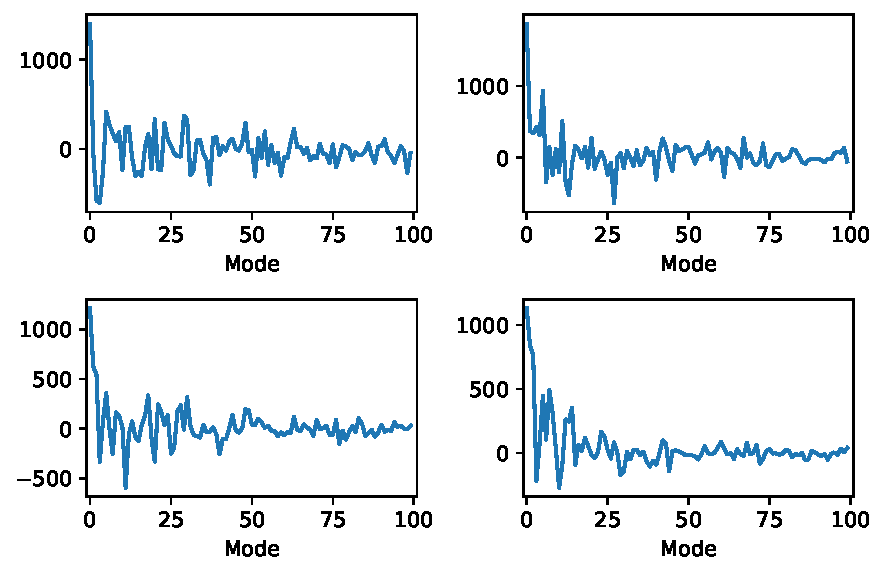
\includegraphics[width=.48\textwidth]{svd_spectrum.pdf}
        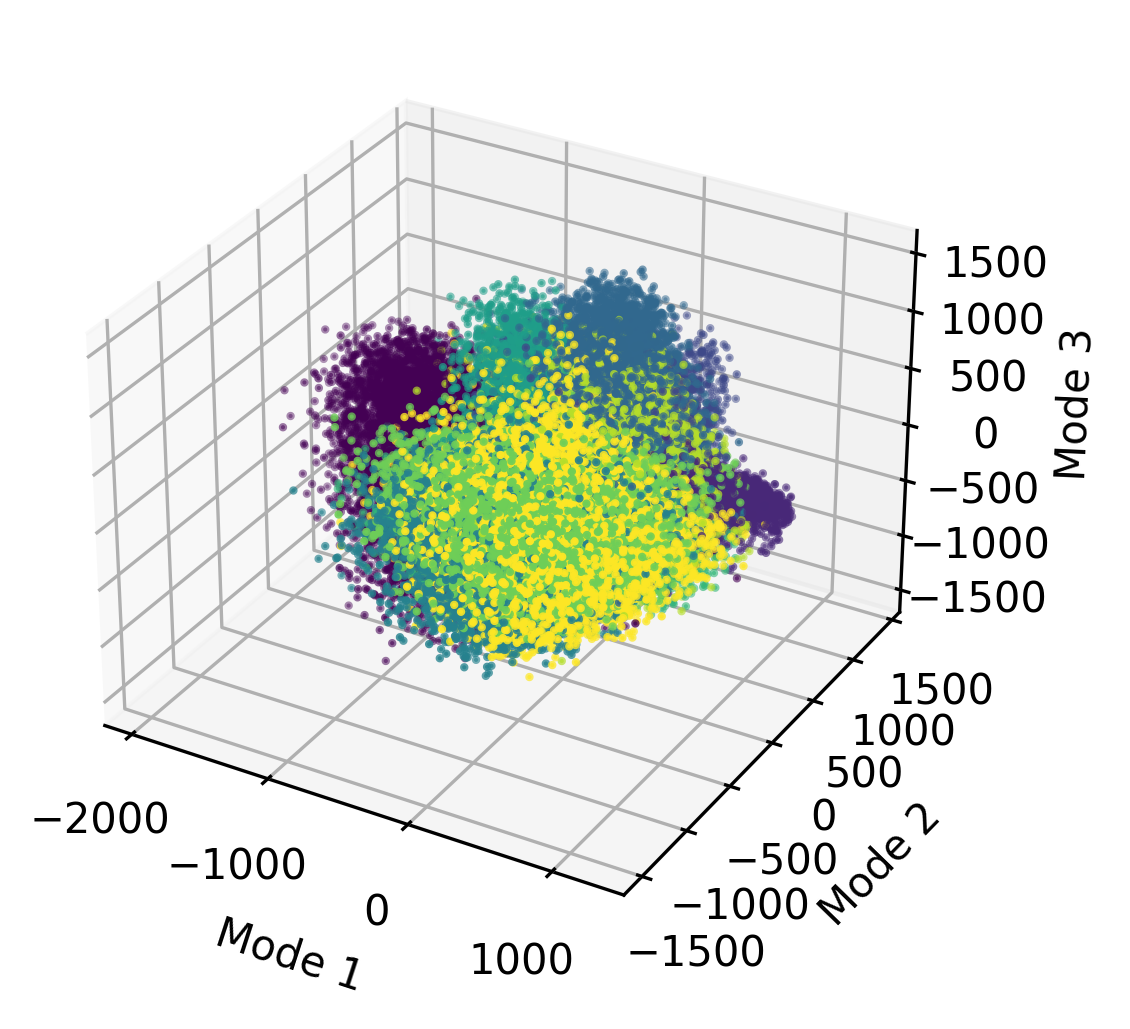
\includegraphics[width=.48\textwidth]{svd_projection.png}
        \caption{\label{fig:projection} Left: 4 Examples of the spectrum of
        the digit samples in the SVD modes. Right) All of the digit samples
        projected onto the 2nd, 3rd and 4th SVD modes. Each digit is colored
        differently.}
    \end{figure}

    It is not necessary to use the full set of modes. Figure \ref{fig:modes}
    plots the total fraction of mode power remaining after $N$ modes are kept.
    By 100 modes, $98\%$ of the power has already been collected. If you
    truncate there, the numbers are still easily readable.

    \begin{figure}[tbp]
        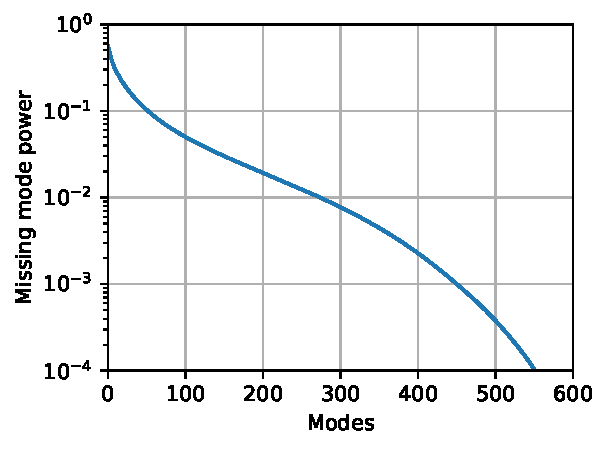
\includegraphics[width=.48\textwidth]{mode_frac.pdf}
        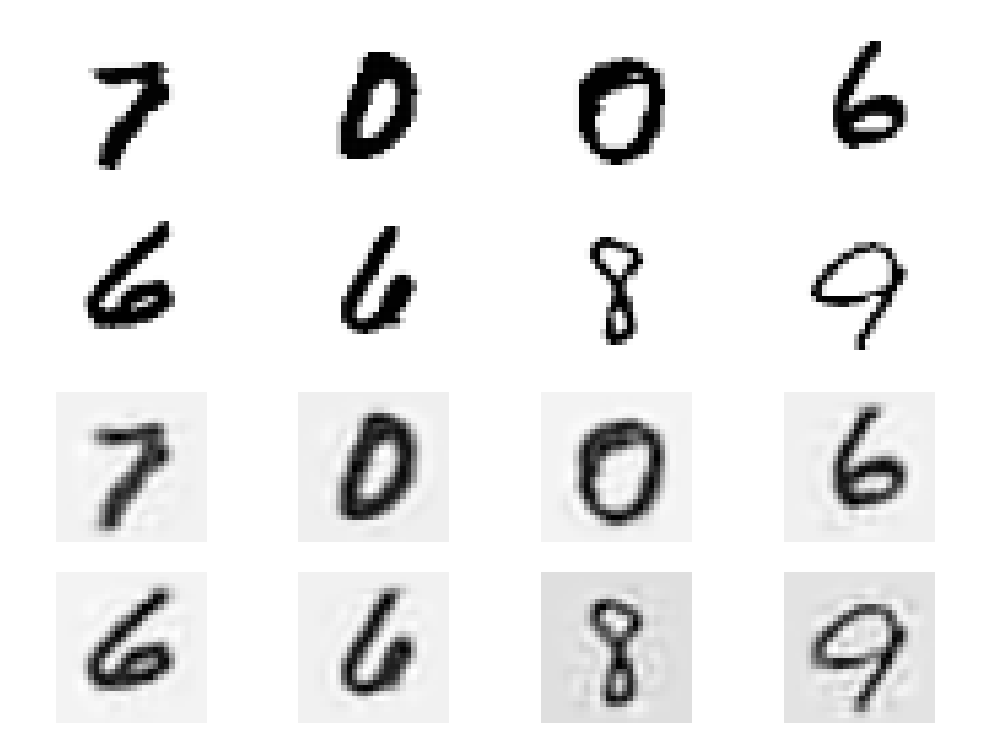
\includegraphics[width=.48\textwidth]{reduced_dim.png}
        \caption{\label{fig:modes} Left: The fraction of total power that is
        still not included after N modes are included. Right: On top are 8
        selected digit samples, and on the bottom are the same digits,
        represented with 100 SVD modes.}
    \end{figure}

    Once in the reduced order modes, LDA is applied identify between pairs of
    digits. Each pair is trained using 2000 samples of the digits. The error
    rate is reported in firgure \ref{fig:lda}. 4 and 7 were the easiest to
    differentiate and 3 and 5 the hardest. I use this to inform
    the sets of 3 digits for the 3 classification test. The first set is
    composed of numbers that were all easily distinguised, 0, 2 and 8. This is
    the best case test. The more sifficult test uses 3 commonly confused numbers,
    0, 4, 5. For the easy set the error rate was 35\% and for the difficult set
    the error rate was 40\%. This is much better than chance, but I wouldn't
    stake my postage delivery on it.

    \begin{figure}[tbp]
        \centering
        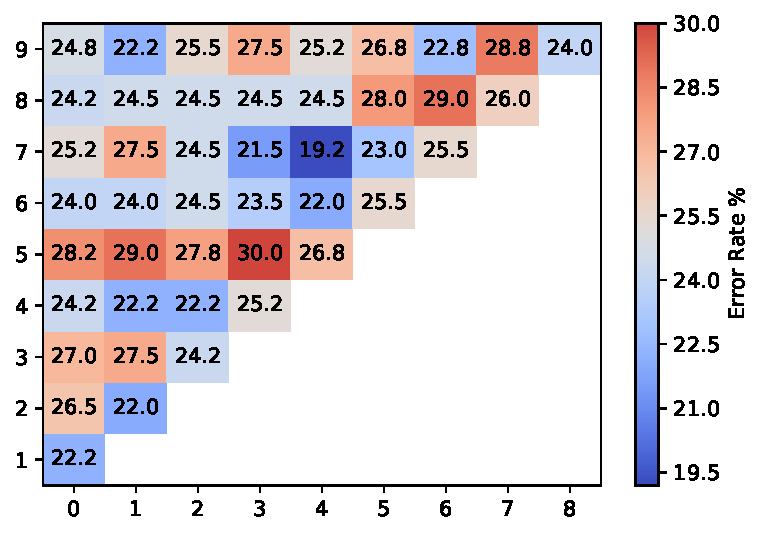
\includegraphics[width=.49\textwidth]{LDA-digits_conf.pdf}
        \caption{\label{fig:lda} For all pairings of digits, the error rate
        of LDA differentiating the two.}
    \end{figure}

    The same test differentiating between all combinations of digit pairs is
    preformed again with two more advanced alogorithms. The error rates are
    presented in fig \ref{fig:other_models}. Both models preform much better
    than LDA, but SVD is the clear winner. Both models struggle with the oairs
    (5, 3) and (5, 8). The decision tree struggles more with (4, 9).

    \begin{figure}[tbp]
        \centering
        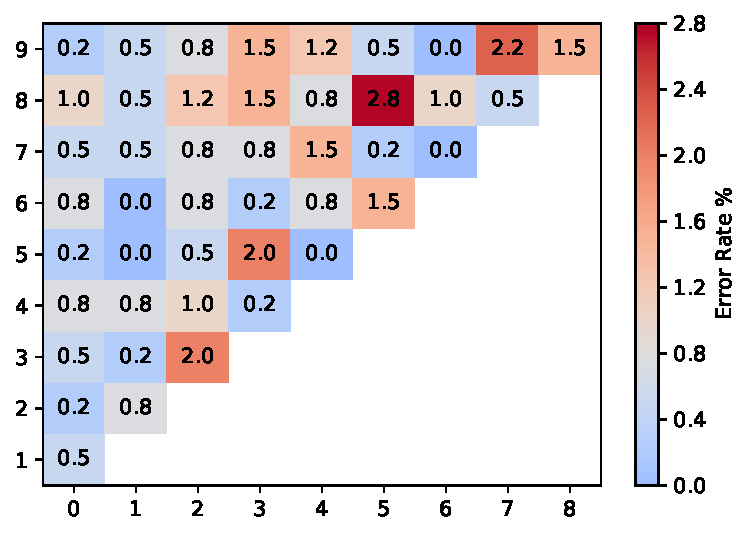
\includegraphics[width=.49\textwidth]{SVC-digits_conf.pdf}
        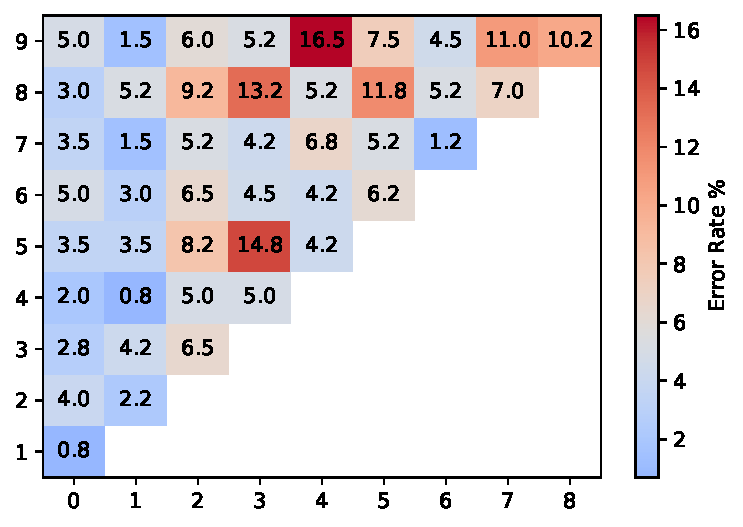
\includegraphics[width=.49\textwidth]{DecisionTreeClassifier-digits_conf.pdf}
        \caption{\label{fig:other_models} For all pairings of digits, the error
        rate differentiating the two. On the left using SVM and the right a
        decision tree.}
    \end{figure}

    When applied to all 10 digits, some of these features persist. The 9 and 4
    confusion severely hurts the ability of the decision tree to correctly label
    both of those digits. Again SVM preforms better, scoring in the high 90s
    for most digits.
    % 10 digit SVM performance
    % 10 digit Decision Tree performance
    \begin{figure}[tbp]
        \centering
        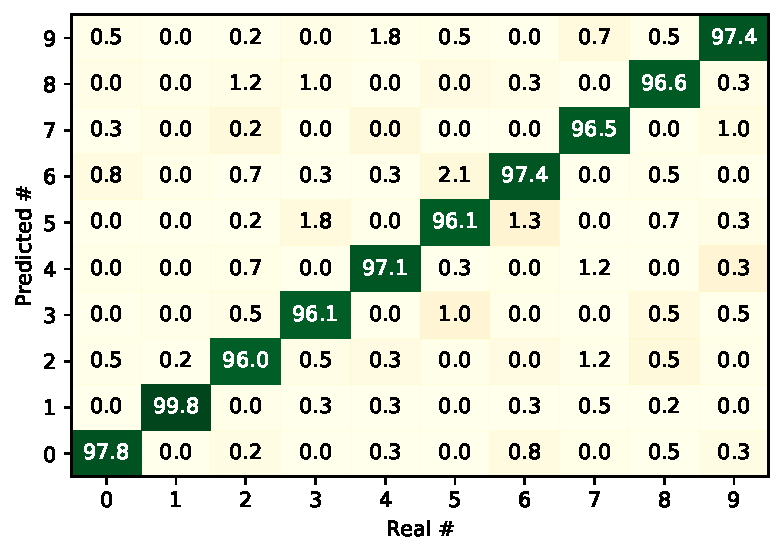
\includegraphics[width=.49\textwidth]{SVC-classification.pdf}
        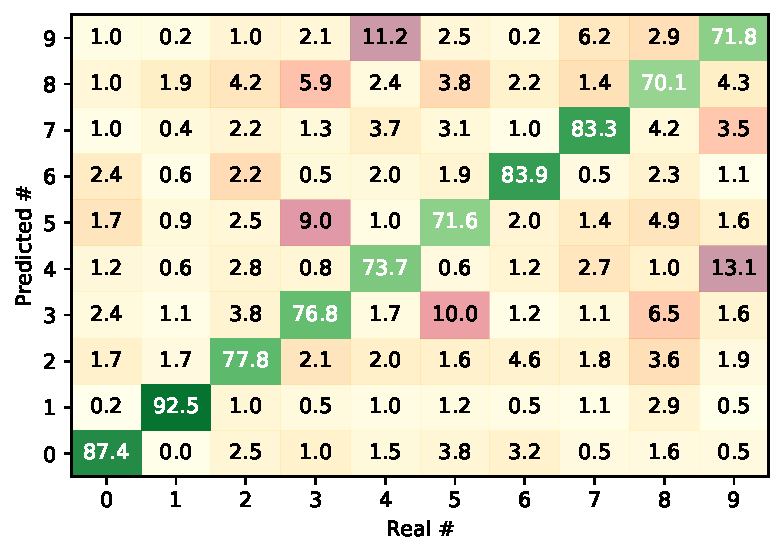
\includegraphics[width=.49\textwidth]{DecisionTreeClassifier-classification.pdf}
        \caption{\label{fig:ten-digit} For the correct digit, the percetage
        that it was identified as. On the left using SVM and the right a
        decision tree.}
    \end{figure}

    \section{Summary and Conclusions}
    Digit differentiation is explored with three different algorithms. SVMs are
    the best performer on this data set. The biggest take away from this project
    for me is how easy it is to implement models using scikit-learn. There is no
    reason that these shouldn't be tried out on data sets in the research.

    \bibliographystyle{ieeetr}
    \bibliography{bibliography}

    \FloatBarrier
    \newpage
    \appendix
    Here is a \href{https://github.com/bagriffith/AMATH582/tree/main/HW4}
    {link to the Github repository for this project}.
    \section{Python Functions}
    % Use PyDoc to generate
    \subsection{dmd}

\subsubsection{dmd}

\begin{Shaded}
\begin{Highlighting}[]
\NormalTok{dmd(X2, u, s, vh)}
\end{Highlighting}
\end{Shaded}

Returns the DMD modes and complex frequencies for the system.

\textbf{Arguments}:

\begin{itemize}
\tightlist
\item
  \texttt{X2} \emph{array-like} - The X\_2\^{}M matrix
\item
  \texttt{u} \emph{array-like} - The U matrix of the X\_1\^{}M-1 SVD
\item
  \texttt{s} \emph{array-like} - The s array of the X\_1\^{}M-1 SVD
\item
  \texttt{vh} \emph{array-like} - The vh matrix of the X\_1\^{}M-1 SVD
\end{itemize}

\textbf{Returns}:

\begin{itemize}
\tightlist
\item
  \texttt{ndarray} - Array of complex frequencies for DMD modes
\item
  \texttt{ndarray} - Matrix with rows of the DMD modes
\end{itemize}

\subsubsection{x\_dmd}

\begin{Shaded}
\begin{Highlighting}[]
\NormalTok{x_dmd(t, psi, w, b)}
\end{Highlighting}
\end{Shaded}

The DMD approximation of x(t).

\textbf{Arguments}:

\begin{itemize}
\tightlist
\item
  \texttt{t} \emph{float} - The time in frames
\item
  \texttt{psi} \emph{array-like} - Matrix with rows of the DMD modes
\item
  \texttt{w} \emph{array-like} - Array of complex frequencies for DMD
  modes
\item
  \texttt{b} \emph{array-like} - Array of initial values of the DMD
  modes
\end{itemize}

\textbf{Returns}:

\begin{itemize}
\tightlist
\item
  \texttt{ndarray} - DMD approximation of pixels at t
\end{itemize}

\subsubsection{frame\_bg\_sep}

\begin{Shaded}
\begin{Highlighting}[]
\NormalTok{frame_bg_sep(t, X, psi, w, b)}
\end{Highlighting}
\end{Shaded}

Separate the forground and background of frame t

\textbf{Arguments}:

\begin{itemize}
\tightlist
\item
  \texttt{t} \emph{int} - The time in frames
\item
  \texttt{psi} \emph{array-like} - Matrix with rows of the DMD modes
\item
  \texttt{w} \emph{array-like} - Array of complex frequencies for DMD
  modes
\item
  \texttt{b} \emph{array-like} - Array of initial values of the DMD
  modes
\end{itemize}

\textbf{Returns}:

\begin{itemize}
\tightlist
\item
  \texttt{ndarray} - Foreground array
\item
  \texttt{ndarray} - Background array
\end{itemize}

\subsubsection{show\_frame}

\begin{Shaded}
\begin{Highlighting}[]
\NormalTok{show_frame(frame, shape, path_out)}
\end{Highlighting}
\end{Shaded}

Plot the frame provided.

\textbf{Arguments}:

\begin{itemize}
\tightlist
\item
  \texttt{frame} \emph{array-like} - 1 D array of pixels
\item
  \texttt{shape} \emph{tuple} - The shape of the image (pixels\_y,
  pixels\_x)
\item
  \texttt{path\_out} \emph{str} - Path to save figure to
\end{itemize}

\subsection{svd}

\subsubsection{plot\_n\_modes}

\begin{Shaded}
\begin{Highlighting}[]
\NormalTok{plot_n_modes(X, V, n, shape, path_out)}
\end{Highlighting}
\end{Shaded}

Shows the numbers represented with the selected number of SVD modes

\textbf{Arguments}:

\begin{itemize}
\tightlist
\item
  \texttt{X} \emph{array\_like} - Data matrix with rows of images
\item
  \texttt{V} \emph{array\_like} - Matrix with mode vectors as columns
\item
  \texttt{n} \emph{int} - Number of modes to use in the representation
\item
  \texttt{shape} \emph{tuple} - The shape of the image (pixels\_y,
  pixels\_x)
\item
  \texttt{path\_out} \emph{str} - Path to save figure to
\end{itemize}

\subsubsection{plot\_mode\_fraction}

\begin{Shaded}
\begin{Highlighting}[]
\NormalTok{plot_mode_fraction(s, path_out)}
\end{Highlighting}
\end{Shaded}

Plots the fraction of power represented with n modes

\textbf{Arguments}:

\begin{itemize}
\tightlist
\item
  \texttt{s} \emph{array-like} - 1D arrray of the variances of the
  principal components.
\item
  \texttt{path\_out} \emph{str} - Path to save figure to
\end{itemize}

\subsection{loadVid}

\subsubsection{open\_video}

\begin{Shaded}
\begin{Highlighting}[]
\NormalTok{open_video(vid_path)}
\end{Highlighting}
\end{Shaded}

Loads the video matrices

\textbf{Arguments}:

\begin{itemize}
\tightlist
\item
  \texttt{vid\_path} \emph{str} - Path to the video file
\end{itemize}

\textbf{Returns}:

\begin{itemize}
\tightlist
\item
  \texttt{ndarray} - X\_1\^{}M-1
\item
  \texttt{ndarray} - X\_2\^{}M
\end{itemize}


    \section{Python Code}
    \subsection{main.py}
    \inputminted{python}{../code/main.py}

    \subsection{loadmnist.py}
    \inputminted{python}{../code/loadmnist.py}

    \subsection{svd.py}
    \inputminted{python}{../code/svd.py}

    \subsection{evaluation.py}
    \inputminted{python}{../code/evaluation.py}

    \subsection{lda.py}
    \inputminted{python}{../code/lda.py}


\end{document}
